\chapter{Indledning}

\emph{Lithium batterier er højtydende, langtidsholdbare og fås i forskellige former, hvilket gør dem velegnet til mange forskellige applikationer. De har dog ulempen at hvis de ikke overvåges kan de hurtigt forgå eller, i værste fald, kan der opstå farlige situationer. Derfor kan der med fordel anvendes et batteristyresystem til opladning, afladning og vedligeholdelse. Batteristyresystemet overvåger konstant de individuelle celler og batteriet som helhed, for at sikre at parametrene er i orden. I denne rapport vil læseren blive guidet igennem processen bag udviklingen af et batteristyresystem.}

\section{Formål}
Formålet med dette afgangsprojekt er at udarbejde et produkt, der efterviser nogle af de opnåede fagligheder igennem uddannelsen som Diplomingeniør i Elektronik og Datateknik - både teoretisk og praktisk.
\\

Projektet skal afspejle et løsningsforslag fra erhvervslivet, således at slutresultatet er brugbart for Linak, som kan tage udgangspunkt i rapporten til intern evaluering. 

\section{Problemformulering}
Linak er gået ind på markedet indenfor reclinerstole, hvor et nyt aktuatorsystem er under udvikling. Da en batteripakke vil indgå i det samlede system, og den består af en seriekobling af lithium celler, er der brug for et batteristyresystem. Batteristyresystemet (BMS’en) vil sidde mellem batterierne og elektronikken for at styre op- og afladning af batteripakken, samt bidrage med sikkerhed i batteripakken. Problemformuleringen er derfor som følgende:
\\

Et batteristyresystem skal udvikles og realiseres ved hjælp af en microcontroller og integrerede kredse eller transistorer. Det ønskes at være muligt at se aktuel batteristatus via et display eller en konsol samt at batteristyresystemet kan overvåge en seriekobling af fire 18650 Lithium-Ion celler.
\\

Der ønskes svar på følgende problemstillinger: 

\begin{itemize}[noitemsep]
	\item Hvilken topologi af batteristyresystemer egner sig bedst til løsning af de opsatte krav?
	\item Hvordan kan en BMS opbygges ved brug af en integreret batteriovervågningskreds?
	\item Hvordan kan en BMS opbygges uden brug af en integreret batteriovervågningskreds? 
	\item Hvordan fremstilles software til kontrol af en batteripakke?
	%\item Hvordan konstrueres en prototype for overholdelse af EMC standarden XXXXXX (Radiated Emission etc...)?
\end{itemize}

\section{Projektafgrænsning}
Et batteristyresystem kan realiseres på forskellige måder. I dette projekt vil forskellige topologier blive undersøgt i kapitel \ref{kap:topologi}, hvorefter den bedst egnede, vil blive udviklet og realiseret. 
\\

Under projektet vil to prototyper realiseres af samme topologi. Den ene prototype vil blive opbygget omkring en færdig batteriovervågningskreds, hvor den anden prototype vil realiseres diskret. De to prototyper vil efterfølgende blive sammenlignet i kapitel \ref{kap:sammenligning}.
\\

Formålet med at sammenligne de to versioner er at få et overblik over, hvorvidt det kan betale sig, at købe en færdig batteriovervågningskreds i forhold til kostprisen på hardwaren til en diskret opbygget løsning.


\subsection{Kravspecifikation} \label{afs:kravspecifikation}
I dette afsnit fremstår de opsatte krav til projektet. Kravene er en sammenfatning af selvvalgte og Linaks ønsker til funktionalitet.

\subsubsection{Krav til hardware}
\begin{itemize}[noitemsep]
	\item Batteripakken skal bestå af fire Lithium celler
	\item Afladnings- og kortslutningsbeskyttelse
	\item Max afladestrøm, $I_{out} = 6\ampere$
	\item Max opladestrøm, $I_{in} = 1\ampere$
	\item Balancering under opladning ved flere celler i serie. Balanceringsstrømmen skal minimum være på $I_{bal} = 40\milli\ampere$
	\item Batteripakken skal kunne detektere om den er i oplade eller aflade tilstand
\end{itemize}

\subsubsection{Krav til software}
\begin{itemize}[noitemsep]
	\item "Låsning"\space af yderpunkter på batteriernes afladekurve (Brug af f.eks. 80\% af fuld kapacitet)
	\item Temperaturmålinger af celler for sikker drift \textemdash \space funktionsområde op til $\SI{45}{\celsius}$
	\item Systemet skal have en brugerflade
	\item State of charge (SoC) \textemdash \space Information om cellernes kapacitet skal være tilgængelig for brugeren
	\item Softwaren er en del af produktet og skal overholde ANSI-C (C90) standarden
\end{itemize}

%\section{Løsningsmodel}
%Der har under udvikling af begge prototyper taget udgangspunkt i en løsningsmodel. Den er dog løbende blevet ændret i takt med antallet af iterationer. Den endelige løsningsmodel ses på figur \ref{fig:blokdiagram}.

%\begin{figure}[h]
%	\centering
%	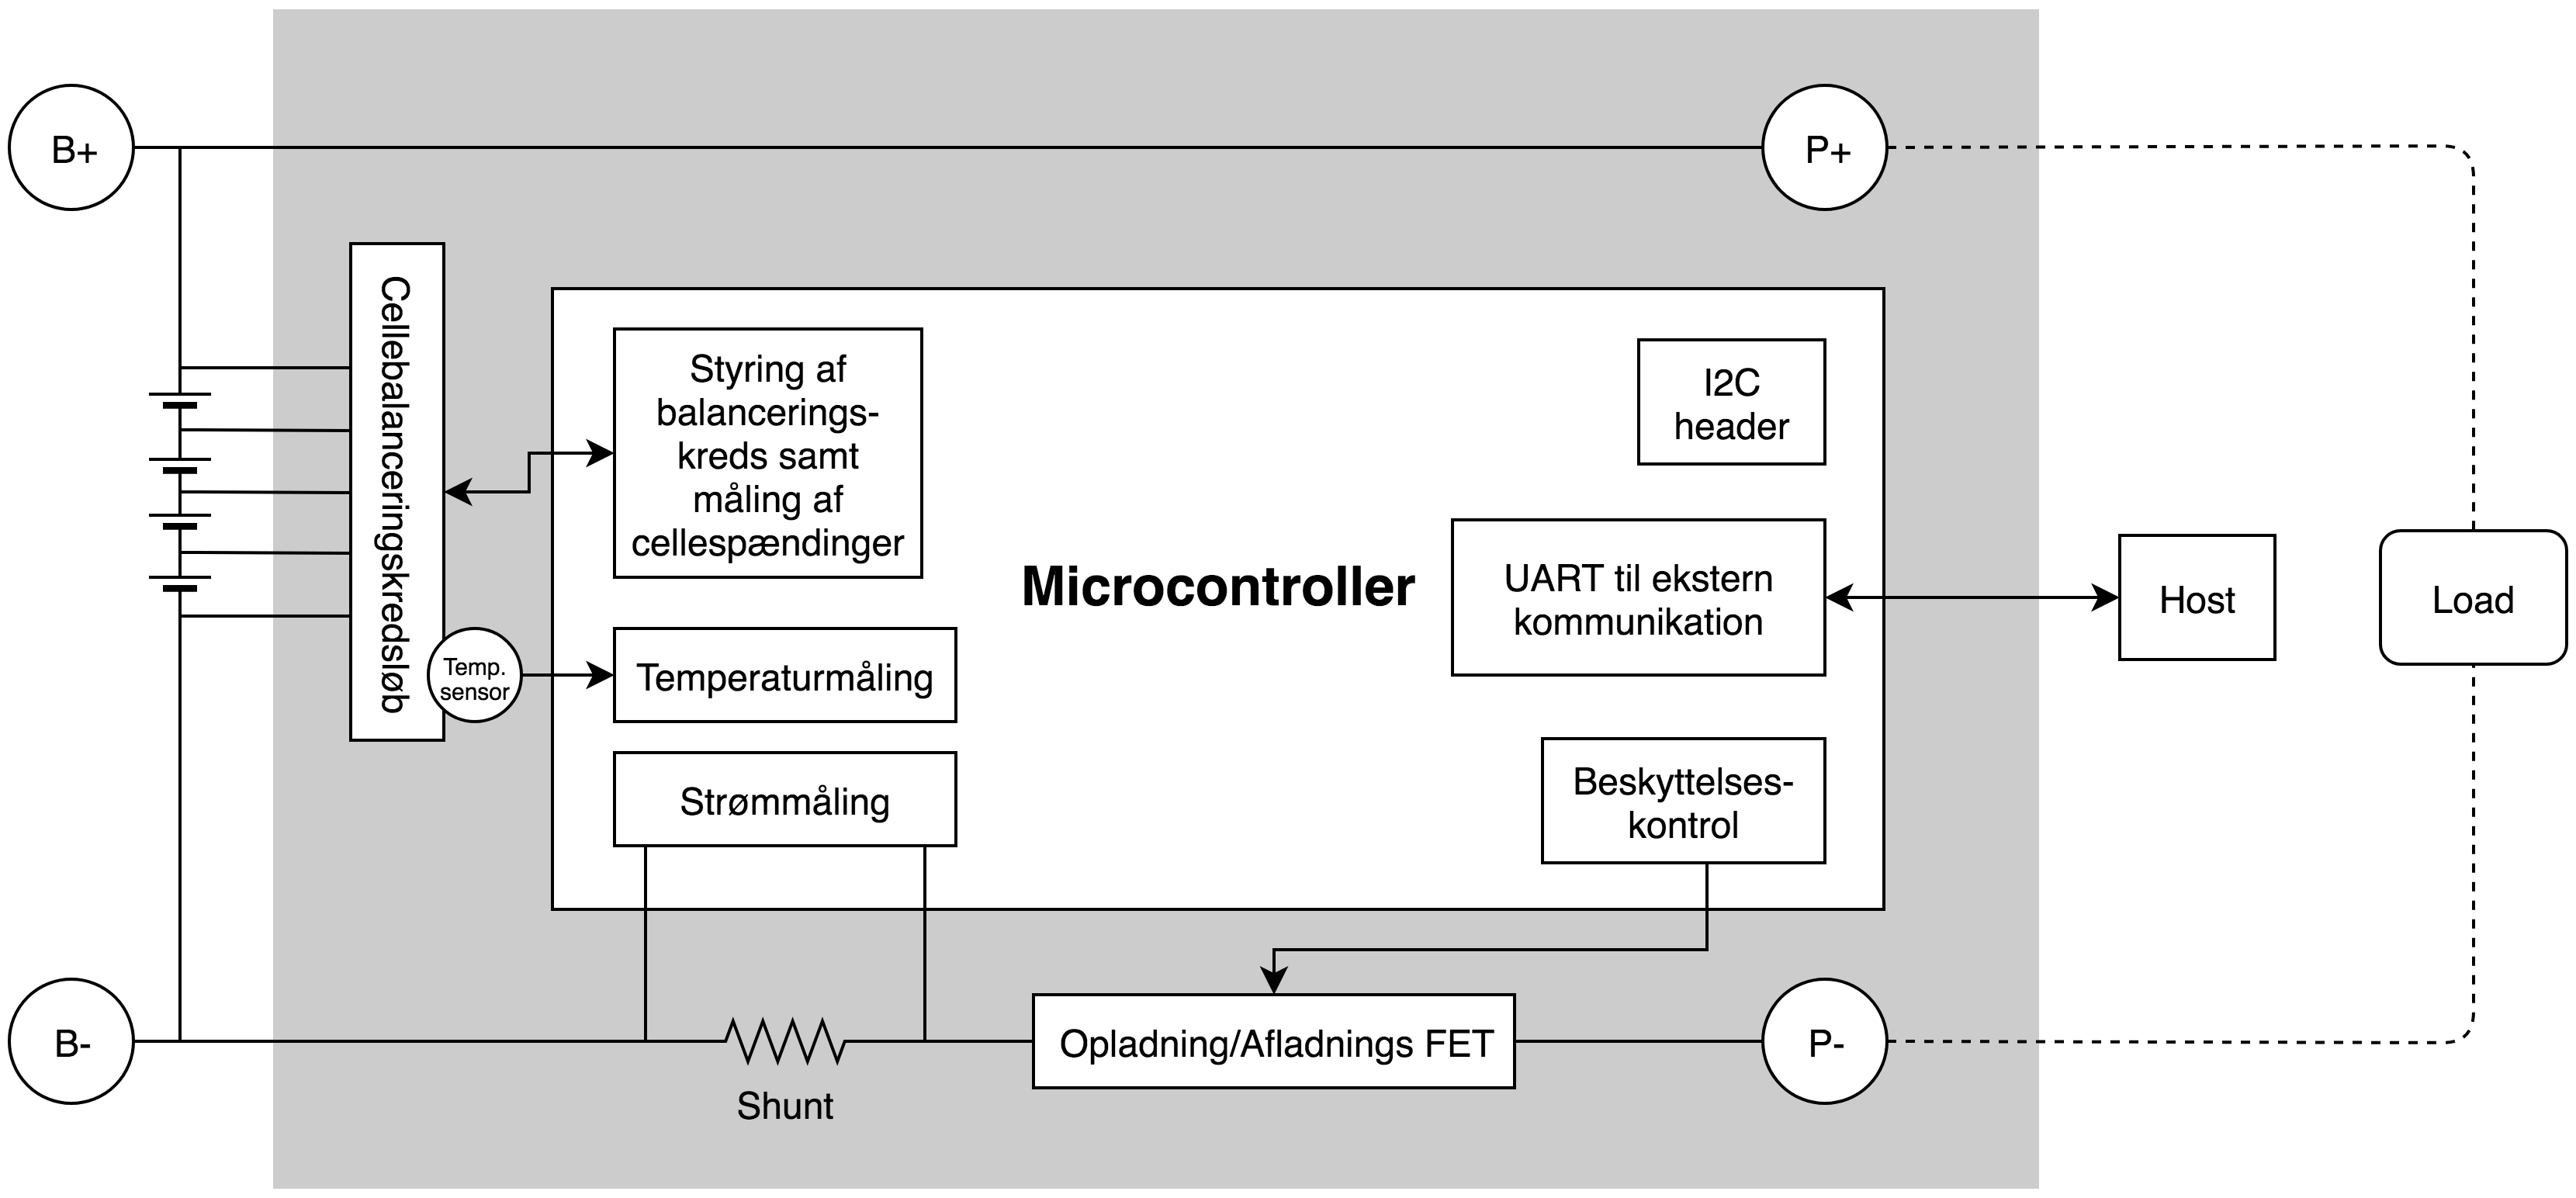
\includegraphics[width=15cm]{billeder/blokdiagram.png}
%	\caption{Løsningsmodel}
%	\label{fig:blokdiagram}
%\end{figure}

\section{Proces- og arbejdsmetode}
Projektarbejdet er delt op i tre faser. Research og forberedelse, udvikling og test, færdiggørelse og konklusion. I research-fasen samles alt relevant information omkring emnet for at opnå en bedre forståelse. Udviklingsfasen tager udgangspunkt i de opsatte krav, hvor flere iterationer vil gennemløbes for at opnå kravene. Den sidste del i projektet vil være en sammenfatning af projektet som helhed.




